\documentclass{article}
%% PACKAGE LOADING

\RequirePackage{geometry}
\RequirePackage[T1]{fontenc}
\RequirePackage{charter}
\RequirePackage{euler}
\RequirePackage{lastpage}
%\RequirePackage[norsk]{babel}
\RequirePackage{enumitem}
\RequirePackage{listings}

\RequirePackage[utf8]{inputenc}     % For utf8 encoded .tex files  % For cross references in pdf
%\RequirePackage[pdftex]{graphicx, hyperref}
\RequirePackage{graphicx}
\RequirePackage{hyperref}
\RequirePackage{color}              % For colouring text  

\hypersetup{colorlinks=true,     
		linkcolor=blue,          % color of internal links (change box color with linkbordercolor)
    citecolor=blue,        % color of links to bibliography
    filecolor=blue,      % color of file links
    urlcolor=blue           % color of external links
		}
\setlist[enumerate]{itemsep=0mm, topsep=5pt, partopsep=0mm, parsep=0mm}
\setlist[enumerate,1]{label=\arabic*., ref=\arabic*}
\setlist[enumerate,2]{label=\arabic*., ref=\arabic*}
\setlist[enumerate,3]{label=\alph*., ref=\alph*}
\setlist[itemize]{itemsep=0mm, topsep=5pt, partopsep=0mm, parsep=0mm}
\setlist[itemize,1]{label=$\bullet$}
\setlist[itemize,2]{label=$\circ$}
\setlist[itemize,3]{label=$\cdot$}
%\RequirePackage[absolute]{textpos}

\usepackage{csvsimple}
\usepackage{booktabs}

\usepackage{gnuplottex}


\definecolor{darkgreen}{rgb}{0,0.5,0}
\definecolor{darkred}{rgb}{0.5,0.0,0}

\lstset{        basicstyle=\ttfamily,
                keywordstyle=\color{blue}\ttfamily,
                stringstyle=\color{darkred}\ttfamily,
                commentstyle=\color{darkgreen}\ttfamily,
}


%Typesetting of C++
\newcommand{\CPP}[0]{{C\nolinebreak[4]\hspace{-.1em}\raisebox{.1ex}{\small\bf +\hspace{-.1em}+\ }}}



%\newcommand{\comment}[1]{\textcolor{blue}{\emph{#1}}}  %% use of the colour and you can see how to use commands with parts \comment{so what}

%% The class files defines these two
%% \newcommand{\NTNU}{Norwegian University for Science and Technology} %

% you can create you one #define like structures using the \newcommand feature
% you can change behaviour using \renewcommand

\newcommand{\com}[1]{{\color{red}#1}} % supervisor comment
%\renewcommand{\com}[1]{} %remove starting % to remove supervisor comments
% This will appear in text \com{Lectures comment} and be visible unless you uncomment
% the renewcommand line.

\newcommand{\todo}[1]{{\color{green}#1}} % items to do
%\renewcommand{\todo}[1]{} %remove starting % to remove items to do

\newcommand{\n}[1]{{\color{blue}#1}} % other comment
%\renewcommand{\n}[1]{} %remove starting % to remove notes

\newcommand{\dn}[1]{} % add the d to a note to say that you have finished with it.

\newcommand{\gj}{NTNU i Gj\o{}vik}






\title{IMT3601 Game Programming - \\ \todo{Your title here}}
\author{Simon McCallum, Marius Nowostawski}
\date{December 2017}


\usepackage{natbib}
\usepackage{graphicx}

\begin{document}

\maketitle


\section{Pitch}
\label{sec:pitch}
This is the short description of the game you developed.  Think of it at what might appear on Steam or on the back of the box of the game.  This could be similar to the pitch you gave the first year students. You could include multiple screen shots.

\begin{figure}[h!]
\centering
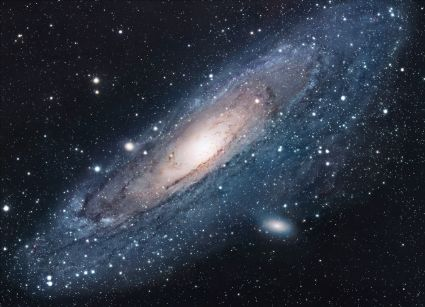
\includegraphics[scale=1.7]{images/universe.jpg}
\caption{Screenshot from Level X }
\label{fig:univerise}
\end{figure}


\section{Team}
\label{sec:team}

\begin{tabular}{lll}
Student         & Role          & Area of Responsibility \\ \hline
Simon McCallum  & Design Lead   & Course overveiw\\
Mariusz Nowostawski & Tech Lead & Netorking \\
Christopher Frantz & Intern     & Population Simulation\\
\end{tabular}

\section{Links}

\todo{In this section you should include the links to the repositories with code and also any executable or videos we should watch}



\section{Implementation}
\label{sec:implementation}

This section describes what you have implemented focusing on what is the most challenging aspects of the development.

\subsection{Development Environment}

What environment you used which might be connected to the section below on technology if the two are linked

\subsection{Technology}

The technology you used to develop the game, the engine or libraries


\subsection{External Dependencies}
Other tools that your game relies on

\subsection{Architecture}
A brief overview of the architecture of the game you made





The subsections should include content on the interesting decisions you had to make and why you made them.  This is an opportunity for you to reflect on the project and what you learnt and why you did what you ended up doing.


\subsection{}
\section{Decisions}

While developing you game you will have made various decisions about the development.  In this section you discuss the decisions you make, why you made them, and would you make the same decision with the information and experience you now have.

You can structure the section like this

\subsection{Perspective}
Working out the way to display the game.  We have a choices of:

\begin{description}
\item[2D] allows simpler assets and lower processing cost
\item[Fake 2.5D] A traditional game look 
\item[3D] requires more assets but looks better
\end{description}

We choose to go with 2.5D iso to give a feel for 3D while keeping the asset list short. We used a game template city builder kit to speed up the development process.  This gave us a 2.5D system as the default view. 

This was a good discussion, as we were able to get the assets form a third party.  We should have gone with the standard perspective rather than the clash of clans 37.5 degrees

\subsection{AI characters}
CityCop needed to simulate a world.  We decided to simulate a village.  This leads to a discussion on how to simulate the the AI

\begin{description}
\item[Desire model] uses a level of desire for each action and lets the sims move about the world based on the desires they have
\item[Random] let the sims move around the world at random 
\item[Scripted] AI would require us to write a path for each of the agents.  Easy to control but time consuming 
\end{description}

We choose to use the Desire model as it would allow us to have a richer environment for future expansions for new levels and scenarios.

In the level of game we finally developed the complexity of the desire model was not obvious.  We could have implemented a purely random system and had a similar experience for the player 



\section{Reflections}

In this section you will need to discuss what was the most difficult aspect of the development process and reflect on what you learnt from those challenges, and from the project as a whole.

The main goal of writing this section is for you to learn by reflecting on what when well and what went badly.  This can be in the form of a Game Postmortem~\footnote{\url{https://blog.codinghorror.com/game-development-postmortems/}} where you describe 5 good things that went better than expected, and 5 bad things and how you would change them.

We are looking for your ability to reflect on the challenges you faces and learn from those challenges.  Why these situations contributed to your learning, and what will you take forward into future projects.

\subsection {The Good}

\subsubsection{Final collaboration}
The final crunch period worked very well.  This section should have enough content to show that you understand why things went well and how you will try to encourage this again.

There should be another 4 things here. If you want you can add more than 5 but not less than 5.

\subsection {The Bad}


\section{ Personal Reflections}
This section describes the individual reflections on learning.

\subsection{Simon McCallum}
The project has been a challenge as the time allocated did not allow me to spend the time I would like to on the project.  I area where I learnt the most was development within Unity.  

\subsection{Mariusz Nowostawski}
...
\section{Conclusion}

What is your summary of the project with a focus on

\section{Learning Outcomes}

What was the most improtatnt things that you learnt during the semester.

``I always thought something was fundamentally wrong with the universe'' \citep{adams1995hitchhiker}



\bibliographystyle{plain}
\bibliography{references}
\end{document}
